
%===================================================================================================
%===================================================================================================
\section{Experiments}
\label{sec:experiments}
%===================================================================================================
%===================================================================================================


Every experiment was conducted with NVIDIA Tesla P40 GPUs with CUDA 10.1.243, each having 22 GiB of memory. For reproducibility, codes for all benchmarks provided in this section is made available in the repository\footnote{Further details available at \href{https://torchgpipe.readthedocs.io/en/stable/benchmarks.html}{this link}.}.
% depth = 5
% num convs per block = 5
% downsample by MaxPool2d
% upsample by Upsampler


%===================================================================================================
\subsection{Effects of Optimization Components}
\label{subsec:ablation-study}

We conducted an experiment to show that every component of {\torchgpipe} is necessary to achieve the maximal efficiency. Starting from the baseline which only has deterministic clock-cycle but no others, each component (backward dependency via \cmtt{Fork} and \cmtt{Join}, non-default streams for copy kernels, and portals for skip connections) is added incrementally. We report the throughput, GPU utilization, and memory usage under each setting to measure how each component contributed to the performance of {\torchgpipe}. We find that addition of each component gives a speed-up, and with all components {\torchgpipe} runs nearly twice as fast as the baseline. Results can be found in \autoref{table:components-ablation}.

We used U-Net for the experiment. Details of the architecture can be found in \autoref{subsubsec:unet-memory} and we set $(B, C)$ to be $(5, 64)$ as in the speed benchmark. In settings without portals, the model is implemented as a fully sequential version where skip connections are encoded as inputs and outputs of layers that they pass through, as described in the symptomatic example of \autoref{subsec:skip}. For the setting with all components, it is implemented with \cmtt{torchgpipe.skip} while the architecture is identical. 

We also visualized per GPU timelines to help understanding each component's role, illustrated in \autoref{fig:unet-timelines}. Explanation for each picture is summarized as follows.

\begin{table*}[t]
    \centering
    \begin{tabular}{ccc|c|c|c|c}
        \multicolumn{3}{c|}{\bf{Optimization components}} & \bf{Throughput} & \bf{Speed up} & \bf{Utilization} & \bf{Memory usage} \\
    \hline
        $\times$   & $\times$ & $\times$ & 30.662/s &     1 & 44\% & 52.2 GiB \\
        Dependency & $\times$ & $\times$ & 41.306/s & 1.347 & 59\% & 19.1 GiB \\
        Dependency & Streams  & $\times$ & 55.191/s & 1.800 & 71\% & 30.0 GiB \\
        Dependency & Streams  & Portals  & 58.477/s & 1.907 & 75\% & 23.5 GiB \\
    \end{tabular}
    \caption{Performance of {\torchgpipe} when optimization components are incrementally added. The U-Net model with $(B, C)=(5, 64)$ is used for the experiment. The batch size and the number of micro-batches are fixed as 128 and 8, respectively. The model is partitioned and placed on four devices via {\torchgpipe}. Here the partition was found manually with the aid of \cmtt{torchgpipe.balance}.}
    \label{table:components-ablation}
    % DataLoader 오버헤드를 완전 배제하기 위해 가짜 입력 사용: 2048x3x192x192x192, 출력은 1 클래스
    % SGD without momentum
\end{table*}

\begin{figure*}[t]
    \centering
    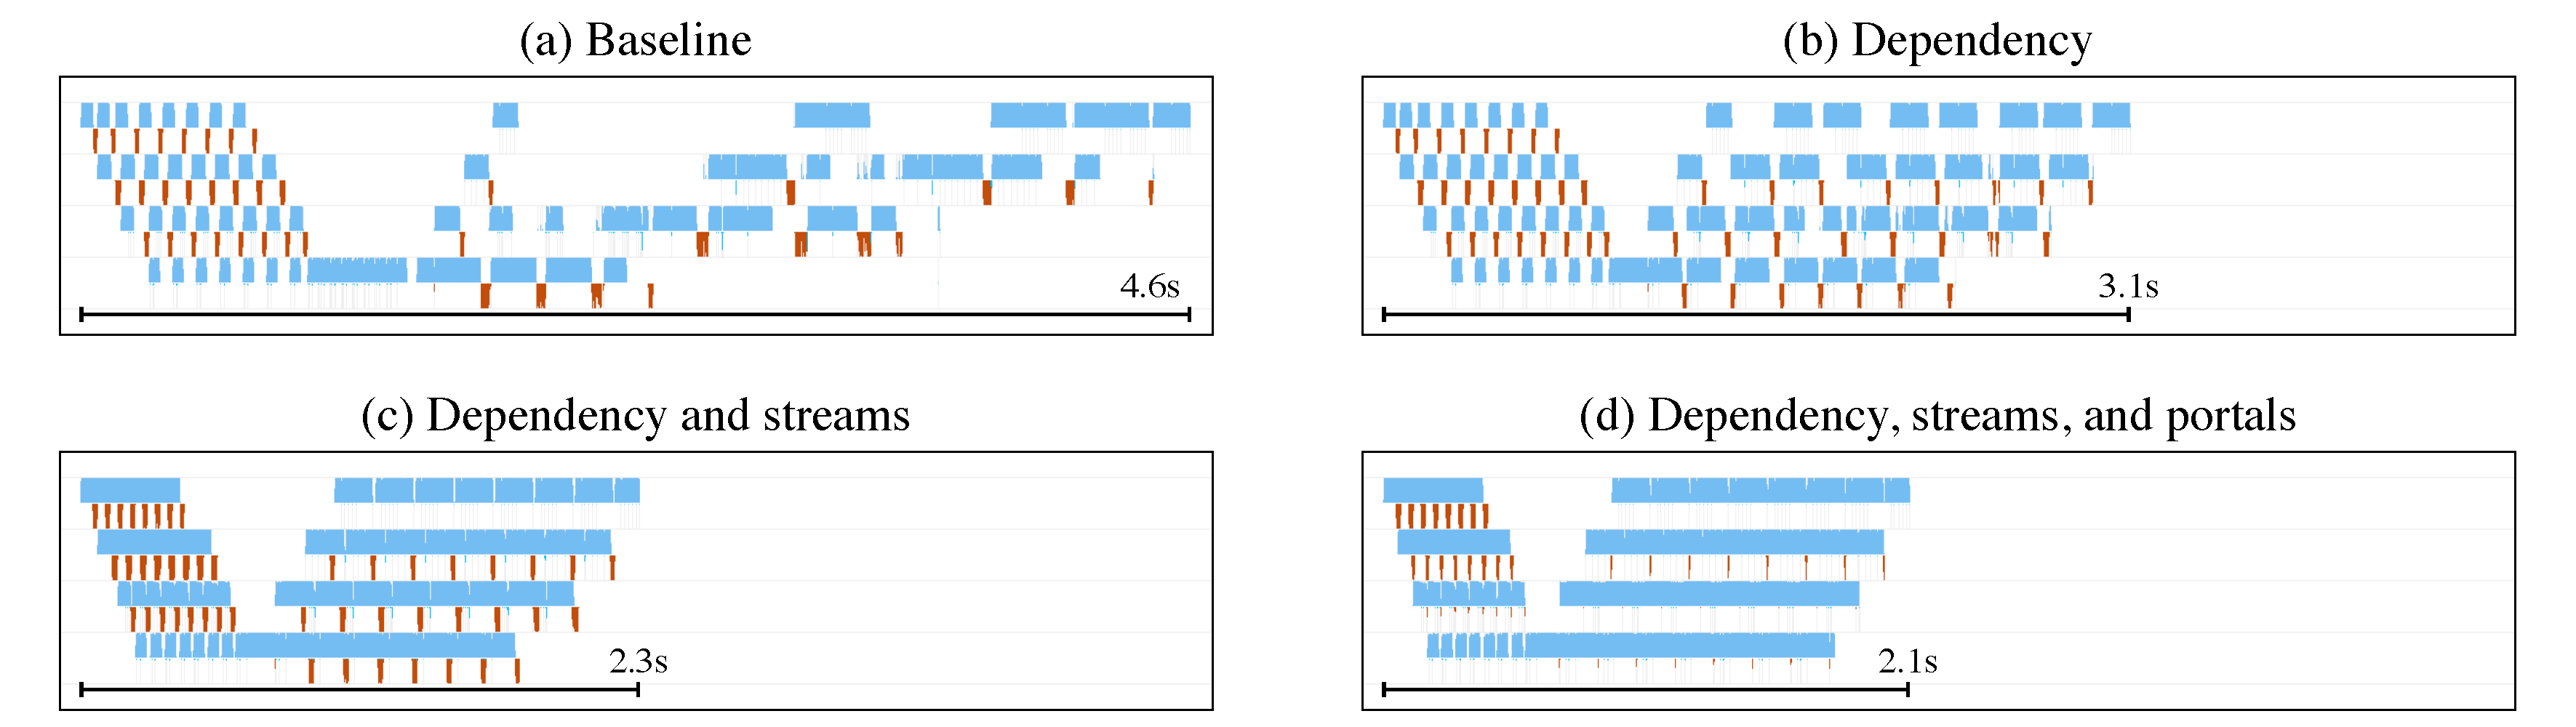
\includegraphics[width=\textwidth]{figures/unet-timelines.pdf}
    \caption{Detailed view of CUDA timeline for each setting in \autoref{table:components-ablation}, profiled with NVIDIA Nsight Systems 2019.5.1.58. Starting from the top, adjacent lanes with blue bars and red bars visualize the timeline per device. Blue bars represent computation kernels while red bars represent device-to-device copy (length proportional to time).}
    \label{fig:unet-timelines}
\end{figure*}

\begin{itemize}
    \item[(a)] By deterministic clock-cycle, all kernels are issued in the correct order during forward pass. It is illustrated by the left part of the timeline. However, without explicit dependency encoded in the computation graph, the autograd engine processes the micro-batches in an uncontrollable order so the timeline is messed up.
    \item[(b)] With backward dependency, kernels are now issued in the correct, deterministic order in backward pass.
    \item[(c)] By using non-default copy streams, copies and computations are now concurrent as illustrated by overlapping blue and red bars.
    \item[(d)] Portals remove unnecessary copies caused by transferring the skipping tensor to all devices in between. This is illustrated by that the length of red bars are reduced compared to (c). 
\end{itemize}


%===================================================================================================
\subsection{Performance Benchmarks}

To demonstrate the efficiency of {\torchgpipe}, we report performance benchmarks similar to that conducted by GPipe \cite{huang2019gpipe}. 

% \subsubsection{ResNet-101 Speed Benchmarks}

% We measured the throughput of ResNet-101 with various number of devices. Naive-1 denotes the baseline without pipeline parallelism nor checkpointing, and Pipeline-1, -2, -4, -8 denotes that the model is trained with {\torchgpipe} with the corresponding number of partitions. To exclude the overhead caused by data loading, we generated a synthesized dataset which consists of 50,000 tensors whose dimension is $3 \times 224 \times 224$. We train the model using plain SGD for 10 epochs and reported the average throughput over the epochs except the first one. The ResNet-101 model we used has a classifier with 1,000 classes at the end, and is re-implemented in a fully sequential form. For each setting, the batch size and the number of micro-batches are chosen to maximize the throughput. 

% In \autoref{table:resnet101-speed}, relative speed-up of pipeline-parallel training against Naive-1 is reported. For reference, we included the speed-up reported in the old version of \cite{huang2019gpipe}. This values are estimated from the chart since exact numbers were not given. We observe that the relative speed-up attained by {\torchgpipe} outperforms that of GPipe, but this might be caused by unknown factors such as balance of the partitions, discrepancy between the implementation, and so on. We emphasize that we included this solely for reference, not to compare it directly with {\torchgpipe}.

\subsubsection{AmoebaNet-D Speed Benchmark}
\label{subsubsec:amoebanetd-speed}
We measured the throughput of AmoebaNet-D with various number of devices. For this, we measured the throughput of the model when {\torchgpipe} is applied, with $n$ partitions and $m$ micro-batches. Here throughput means the number of samples processed per second. 

The experiment is conducted for each pair $(m, n)$ where $m \in \{1, 4, 32\}$ and $n \in \{2, 4, 8\}$. When $m=1$, we used checkpointing to all micro-batches\footnote{{\torchgpipe} does not use checkpointing on the last micro-batch by default, as explained in \autoref{sec:pipeline-parallelism}. This means that no checkpointing is applied when $m=1$.} to make a fair comparison of loss due to checkpointing with \cite{huang2019gpipe}. The model we used is our implementation of a sequential version of AmoebaNet-D in PyTorch\footnote{We tried to make it as close as possible to the model in the official repository of TensorFlow (\href{https://github.com/tensorflow/tpu/tree/master/models/official/amoeba_net}{link}).}.

The model is trained by plain SGD for 10 epochs and reported the average throughput over the epochs except the first one. To exclude the overhead caused by data loading, we used a synthesized dataset which consists of 10,000 images whose dimension is $3 \times 224 \times 224$. For each setting, the batch size and the number of micro-batches are chosen to maximize the throughput. Relative speed-up is calculated against the baseline case $(m, n) = (1, 2)$ and reported in \autoref{table:amoebanetd-speed}. We included the speed-up of GPipe for comparison. 

The relative speed-up of {\torchgpipe} shows similar trend to that of GPipe. We remark that differences in performance reported in \autoref{table:amoebanetd-speed} might be due to many unknown factors such as balance of the partitions, discrepancy between the implementation, difference in devices, and so on. 


\subsubsection{U-Net Memory Benchmark}
\label{subsubsec:unet-memory}

To evaluate the effectiveness of {\torchgpipe} for models with long skip connections, we used U-Net \cite{RonnebergerFB15} for 2-dimensional segmentation. The version of U-Net we used has five down-sampling layers and five up-sampling layers, and two hyper-parameters $B$ and $C$ determining the size of the model. Here $B$ stands for the number of convolution blocks in between down-sampling layers, and $C$ stands for the number of output channels of the first convolution. Channels are doubled after each down-sampling layers (or halved after each up-sampling layers, respectively). Our implementation of U-Net is rather symmetric than the original model proposed in \cite{RonnebergerFB15} for effective balancing.

We conducted an experiment to measure the ability of {\torchgpipe} for training a bigger model. For 1, 2, 4 and 8 GPUs, we found maximum $(B, C)$ to occupy each number of devices. In all settings, the input size is set to $3 \times 192 \times 192$, the output size to $1 \times 192 \times 192$, and the batch size to 32. The total memory usage for training each model is reported in \autoref{table:unet-memory}. Here parameters consumes 8 bytes each for itself and its gradients.

\subsubsection{U-Net Speed Benchmark}
\label{subsubsec:unet-speed}
% 가짜 입력은 10000x3x192x192, 가짜 정답은 1x192x192
We also measured the throughput of U-Net with various number of devices. Naive-1 denotes the baseline without pipeline parallelism nor checkpointing, and Pipeline-1, -2, -4, -8 denotes that the model is trained with {\torchgpipe} with the corresponding number of partitions. The hyper-parameters determining the size of U-Net is set to $(B, C) = (5, 64)$ in this experiment. The batch size, the number of micro-batches ($m$), and the balance to partitions are chosen to maximize the throughput. For each setting, throughput is measured as in \autoref{subsubsec:amoebanetd-speed} except that the image size was $3 \times 192 \times 192$ in this experiment. Result is summarized in \autoref{table:unet-speed}.


\begin{table}[t!]
    \small
    \centering
    \begin{tabular}[t]{c|ccc|ccc}
        \bf{AmoebaNet-D} & \multicolumn{3}{c|}{GPipe \cite{huang2019gpipe}} & \multicolumn{3}{|c}{Ours} \\
    \hline
        $n =$ & 2 & 4 & 8 & 2 & 4 & 8 \\
    \hline
        $m = 1$  &    1 & 1.13 & 1.38 &    1 & 1.00 & 0.93 \\
        $m = 4$  & 1.07 & 1.26 & 1.72 & 1.54 & 1.67 & 2.62 \\
        $m = 32$ & 1.21 & 1.84 & 3.48 & 1.77 & 2.71 & 4.95 \\
    \end{tabular}
    \caption{Speed benchmark on AmoebaNet-D (18, 256). In \cite{huang2019gpipe}, Cloud TPUv3s were used while we used NVIDIA Tesla P40 GPUs in our experiments.}
    \label{table:amoebanetd-speed}
    \vspace{10pt}
    \begin{tabular}[t]{c|c|c|c}
        \bf{U-Net} & ($B$, $C$) & Parameters & Memory usage \\
    \hline
        Naive-1    & (6, 72)   & 362.2M &  20.3 GiB \\
        Pipeline-1 & (11, 128) &  2.21B &  20.5 GiB \\
        Pipeline-2 & (24, 128) &  4.99B &  43.4 GiB \\
        Pipeline-4 & (24, 160) &  7.80B &  79.1 GiB \\
        Pipeline-8 & (48, 160) & 15.82B & 154.1 GiB
    \end{tabular}
    \caption{Memory benchmark on U-Net.}
    \label{table:unet-memory}
    \vspace{10pt}
    \begin{tabular}[t]{c|c|c|c|c}
        \bf{U-Net} & Throughput & Speed up & Batch size & $m$ \\
    \hline
        Naive-1    & 28.500/s &     1 &  40 & $\times$ \\
        Pipeline-1 & 24.456/s & 0.858 &  80 &        2 \\
        Pipeline-2 & 35.502/s & 1.246 & 512 &       32 \\
        Pipeline-4 & 67.042/s & 2.352 & 512 &       16 \\
        Pipeline-8 & 88.497/s & 3.105 & 640 &       40
    \end{tabular}
    \caption{Speed benchmark on U-Net with $(B, C)=(5, 64)$.}
    \label{table:unet-speed}
\end{table}

% \begin{table*}[t]
%     \centering
%     \begin{minipage}[t]{0.35\textwidth}
%         \centering
%         \begin{tabular}[t]{c|c|c}
%             \bf{ResNet-101} & GPipe \cite{huang2019gpipe} & Ours \\
%         \hline
%             Naive-1    &     1 &     1 \\
%             Pipeline-1 & 0.800 & 0.853 \\
%             Pipeline-2 & 1.418 & 1.414 \\
%             Pipeline-4 & 2.182 & 2.774 \\
%             Pipeline-8 & 2.891 & 4.294
%         \end{tabular}
%         \caption{Speed benchmark on ResNet-101.}
%         \label{table:resnet101-speed}
%         % Experiment    Batch size	Number of Micro-batches
%         % Naive-1       118     	N/A
%         % Pipeline-1    220     	2 - 우리 전략은 except_last인데 한 스텝의 메모리를 다 쓰면서 처리량을 올릴 때 마이크로배치 수 2가 유리했다.
%         % Pipeline-2    25000	    1667
%         % Pipeline-4    5632	    256
%         % Pipeline-8    5400	    150
%         % 실제 학습 아님.
%         % 처리량 극대화를 위해 배치크기와 마이크로배치 수를 조절함.
%         % DataLoader 오버헤드를 완전 배제하기 위해 가짜 입력 사용: 50000x3x224x224, 1000 클래스
%         % 10에폭 측정 후 첫 에폭 제외하고 평균 냄.
%         % SGD without momentum
%         % GPipe 논문보다 낫게 나왔지만, 파티션 간 밸런스 등 공개되지 않은 점에 기인했을 수 있음.
%     \end{minipage}
%     \hspace{0.02\textwidth}
%     \begin{minipage}[t]{0.55\textwidth}
%         \centering
%         \begin{tabular}[t]{c|ccc|ccc}
%             \bf{AmoebaNet-D} & \multicolumn{3}{c|}{GPipe \cite{huang2019gpipe}} & \multicolumn{3}{|c}{Ours} \\
%         \hline
%             $n =$ & 2 & 4 & 8 & 2 & 4 & 8 \\
%         \hline
%             $m = 1$  &     1 & 1.130 & 1.380 &     1 & 1.004 & 0.932 \\
%             $m = 4$  & 1.070 & 1.260 & 1.720 & 1.539 & 1.666 & 2.621 \\
%             $m = 32$ & 1.210 & 1.840 & 3.480 & 1.773 & 2.709 & 4.953 \\
%         \end{tabular}
%         \caption{Speed benchmark on AmoebaNet-D (18, 256).}
%         \label{table:amoebanetd-speed}
%         % Experiment	Batch size	Number of Micro-batches	Checkpoint
%         % k2m1      	96  	1	always
%         % k2m4	        256 	4	except_last
%         % k2m32	        1280	32	except_last
%         % k4m1      	160     1	always
%         % k4m4	        360     4	except_last
%         % k4m32	        1152	32	except_last
%         % k8m1	        196	    1	always      
%         % k8m4	        480	    4	except_last
%         % k8m32	        1280	32	except_last
%         % 실제 학습 아님.
%         % 처리량 극대화를 위해 배치크기를 조절함.
%         % DataLoader 오버헤드를 완전 배제하기 위해 가짜 입력 사용: 10000x3x224x224 (ResNet-101에서보다 적음), 1000 클래스
%         % 마이크로배치 1개일 땐 체크포인팅의 속도 손해를 원 논문과 비교하기 위해 except_last 대신 always 사용.
%         % 10에폭 측정 후 첫 에폭 제외하고 평균 냄.
%         % SGD without momentum
%         % GPipe 논문보다 낫게 나왔지만, 파티션 간 밸런스 등 공개되지 않은 점에 기인했을 수 있음.
%     \end{minipage}
% \end{table*}

% \begin{table*}[t]
%     \centering
%     \begin{tabular}[t]{c|c|c|c|c}
%         \bf{U-Net} & Throughput & Speed up & Batch size & Micro-batches \\
%     \hline
%         Naive-1    & 28.500/s &     1 &  40 & $\times$ \\
%         Pipeline-1 & 24.456/s & 0.858 &  80 &        2 \\
%         Pipeline-2 & 35.502/s & 1.246 & 512 &       32 \\
%         Pipeline-4 & 67.042/s & 2.352 & 512 &       16 \\
%         Pipeline-8 & 76.802/s & 2.695 & 512 &       32
%     \end{tabular}
%     \caption{Speed benchmark on customized U-Net.}
%     \label{table:unet-speed}
%     % 가짜 입력은 10000x3x192x192, 가짜 정답은 1x192x192
%     % Pipeline-8에서 스킵텐서 복사가 중간 레이어의 연산보다 
% \end{table*}

% \begin{table*}[t]
%     \centering
%     \begin{tabular}[t]{c|c|c|c|c}
%         \bf{U-Net} & ($B$, $C$) & Parameters & Model Memory & Peak Activation Memory \\
%     \hline
%         Naive-1    & (6, 72)   & 362.2M &   2.70 GB & 18.85 GB &
%         Pipeline-1 & (11, 128) &  2.21B &  16.49 GB &  3.98 GB &
%         Pipeline-2 & (24, 128) &  4.99B &  37.21 GB &  6.40 GB &
%         Pipeline-4 & (24, 160) &  7.80B &  58.14 GB & 20.92 GB &
%         Pipeline-8 & (48, 160) & 15.82B & 117.88 GB & 36.19 GB &
%     \end{tabular}
%     \caption{Memory benchmark on customized U-Net. The batch size is fixed as 32.}
%     \label{table:unet-memory}
%     % 가짜 입력은 32x3x192x192, 가짜 정답은 1x192x192
%     % Pipeline-8에서 스킵텐서 복사가 중간 레이어의 연산보다 
% \end{table*}